\documentclass{report}
\usepackage[table,xcdraw]{xcolor}
\usepackage{tikz}
\usepackage{fancyhdr}
\usepackage[utf8]{vietnam}
\usepackage{hyperref} % Hyperlink
\usepackage{parskip}
\usepackage[left=2cm,right=2cm,top=2cm,bottom=2cm]{geometry}
\usepackage{listings}
\usepackage{color}
\usetikzlibrary{calc}
\usepackage{titlesec} % Change section font
\usepackage{multirow}
\usepackage{graphicx}
\usepackage{algorithm,algorithmic}
\usepackage{multicol}
\usepackage{setspace}
\usepackage{pdfpages}
\usepackage{lscape}
\usepackage{longtable}

% ========== [LANGUAGE] ==========
\def\lang{1} % 0 == English, 1 == Vietnamese

\ifnum\lang = 0
    \usepackage[english]{babel}
\fi
% ========== END OF [LANGUAGE] ==========
\definecolor{mygreen}{rgb}{0,0.6,0}
\definecolor{mygray}{rgb}{0.5,0.5,0.5}
\definecolor{mymauve}{rgb}{0.58,0,0.82}
 
%Customize a bit the look
\lstset{ %
backgroundcolor=\color{white}, % choose the background color; you must add \usepackage{color} or \usepackage{xcolor}
basicstyle=\footnotesize, % the size of the fonts that are used for the code
breakatwhitespace=false, % sets if automatic breaks should only happen at whitespace
breaklines=true, % sets automatic line breaking
captionpos=b, % sets the caption-position to bottom
commentstyle=\color{mygreen}, % comment style
deletekeywords={...}, % if you want to delete keywords from the given language
escapeinside={\%*}{*)}, % if you want to add LaTeX within your code
extendedchars=true, % lets you use non-ASCII characters; for 8-bits encodings only, does not work with UTF-8
frame=single, % adds a frame around the code
keepspaces=true, % keeps spaces in text, useful for keeping indentation of code (possibly needs columns=flexible)
keywordstyle=\color{blue}, % keyword style
% language=Octave, % the language of the code
morekeywords={*,...}, % if you want to add more keywords to the set
numbers=left, % where to put the line-numbers; possible values are (none, left, right)
numbersep=5pt, % how far the line-numbers are from the code
numberstyle=\tiny\color{mygray}, % the style that is used for the line-numbers
rulecolor=\color{black}, % if not set, the frame-color may be changed on line-breaks within not-black text (e.g. comments (green here))
showspaces=false, % show spaces everywhere adding particular underscores; it overrides 'showstringspaces'
showstringspaces=false, % underline spaces within strings only
showtabs=false, % show tabs within strings adding particular underscores
stepnumber=1, % the step between two line-numbers. If it's 1, each line will be numbered
stringstyle=\color{mymauve}, % string literal style
tabsize=2, % sets default tabsize to 2 spaces
title=\lstname % show the filename of files included with \lstinputlisting; also try caption instead of title
}
%END of listing package%
 
\definecolor{darkgray}{rgb}{.4,.4,.4}
\definecolor{purple}{rgb}{0.65, 0.12, 0.82}
 
%define Javascript language
\lstdefinelanguage{JavaScript}{
keywords={typeof, new, true, false, catch, function, return, null, catch, switch, var, if, in, while, do, else, case, break},
keywordstyle=\color{blue}\bfseries,
ndkeywords={class, export, boolean, throw, implements, import, this},
ndkeywordstyle=\color{darkgray}\bfseries,
identifierstyle=\color{black},
sensitive=false,
comment=[l]{//},
morecomment=[s]{/*}{*/},
commentstyle=\color{purple}\ttfamily,
stringstyle=\color{red}\ttfamily,
morestring=[b]',
morestring=[b]"
}
 
\lstset{
language=JavaScript,
extendedchars=true,
basicstyle=\footnotesize\ttfamily,
showstringspaces=false,
showspaces=false,
numbers=left,
numberstyle=\footnotesize,
numbersep=9pt,
tabsize=2,
breaklines=true,
showtabs=false,
captionpos=b
}




\begin{document}

% ========== [TITLE PAGE] ==========
\begin{titlepage}

\begin{tikzpicture}[overlay,remember picture]
\draw[line width=4pt]
    ($ (current page.north west) + (1cm,-1cm) $)
    rectangle
    ($ (current page.south east) + (-1cm,1cm) $);
\draw[line width=1.5pt]
    ($ (current page.north west) + (1.2cm,-1.2cm) $)
    rectangle
    ($ (current page.south east) + (-1.2cm,1.2cm) $);
\end{tikzpicture}


\begin{center}
% Upper part of the page
\ifnum\lang = 0
    \textbf{\Large UNIVERSITY OF SCIENCE}\\[0.2cm]
    \textbf{\Large FACULTY OF INFORMATION TECHNOLOGY}\\
\else
    \textbf{\Large TRƯỜNG ĐẠI HỌC KHOA HỌC TỰ NHIÊN}\\
    \textbf{\Large KHOA CÔNG NGHỆ THÔNG TIN}\\
\fi

% University Logo
\begin{figure}[!h]
    \centering
    
\includegraphics[width=8cm, height=8cm]{img/KHTN.png}
\end{figure}

% Title
\rule{\textwidth}{1pt} \\[0.4cm]
{\huge \bfseries ĐỒ ÁN CUỐI KÌ - NHÓM 10}\\[0.4cm]
\textsc{\Large VẬT LÝ CHO CNTT}
\rule{\textwidth}{1pt} \\[1cm]

% Student name
\begin{center}
    \textbf{\Large TRIỆU NHẬT MINH - 21127112}\\
    \textbf{\Large BÙI ĐỖ DUY QUÂN - 21127141}\\
    \textbf{\Large HOÀNG ĐỨC VIỆT - 21127203}\\[3cm]
\end{center}

% Advisor name
\begin{center}
    \ifnum\lang = 0
        \textbf{\Large Lecturers: \\[0.2cm]}
    \else
        \textbf{\Large Giảng viên hướng dẫn: \\[0.2cm]}
    \fi
    \Large{Cao Xuân Nam\\[0.2cm] Đặng Hoài Thương}
\end{center}
\vfill

% Bottom of the page
\ifnum\lang = 0
    \selectlanguage{english} 
\fi
{\large \today}
\end{center}
\end{titlepage}
% ========== END [TITLE PAGE] ==========





% ========== [HEADER AND FOOTER] ==========
\pagestyle{fancy}
\setlength{\headheight}{0.5cm}
\fancyhf{}
\lhead{\textbf{Đồ án cuối kì}}
\rhead{\textbf{Vật lý cho CNTT}}
\ifnum\lang = 0
    \rfoot{Page \thepage}
\else
    \rfoot{Trang \thepage}
\fi
% ========== END [HEADER AND FOOTER] ==========





% ========== [TABLE OF CONTENTS] ==========
\Large
\tableofcontents
\thispagestyle{fancy} % Fix footer and header
\vfill
\pagebreak
% ========== END [TABLE OF CONTENTS] ==========





% ========== [SECTION NUMBERING] ==========
\setcounter{secnumdepth}{5} % Section numbering depth 

\renewcommand\thesection{\arabic{section}} % Section start from 1,2,3...
\renewcommand\thesubsection{\thesection.\arabic{subsection}} % Subsection start from 1,2,3,...
\renewcommand\thesubsubsection{\alph{subsubsection}} 

\titleformat*{\section}{\Large\bfseries}
\titleformat*{\subsection}{\Large\bfseries}
\titleformat*{\subsubsection}{\Large\bfseries}
% ========== END [SECTION NUMBERING] ==========





% ========== [MAIN CONTENT] ==========
\section{Thông tin nhóm}
Thứ tự nhóm: Nhóm 10 \par
Danh sách thành viên:
\begin{itemize}
    \item Triệu Nhật Minh - 21127112
    \item Bùi Đỗ Duy Quân - 21127141
    \item Hoàng Đức Việt - 21127203
\end{itemize}

\section{Sản phẩm}
\subsection{Tên sản phẩm}
Thiết bị hỗ trợ sử dụng điện thông minh trong phòng

\subsection{Mô tả toàn chức năng của hệ thống}
\subsubsection{Hình ảnh sản phẩm}
Trong đồ án này, nhóm đã chọn thực hiện giả lập sản phẩm trên nền tảng \textbf{Wokwi} và dưới đây là hình ảnh các thiết bị và mạch nhóm đã thiết kế.
\begin{figure}[!h]
    \centering
    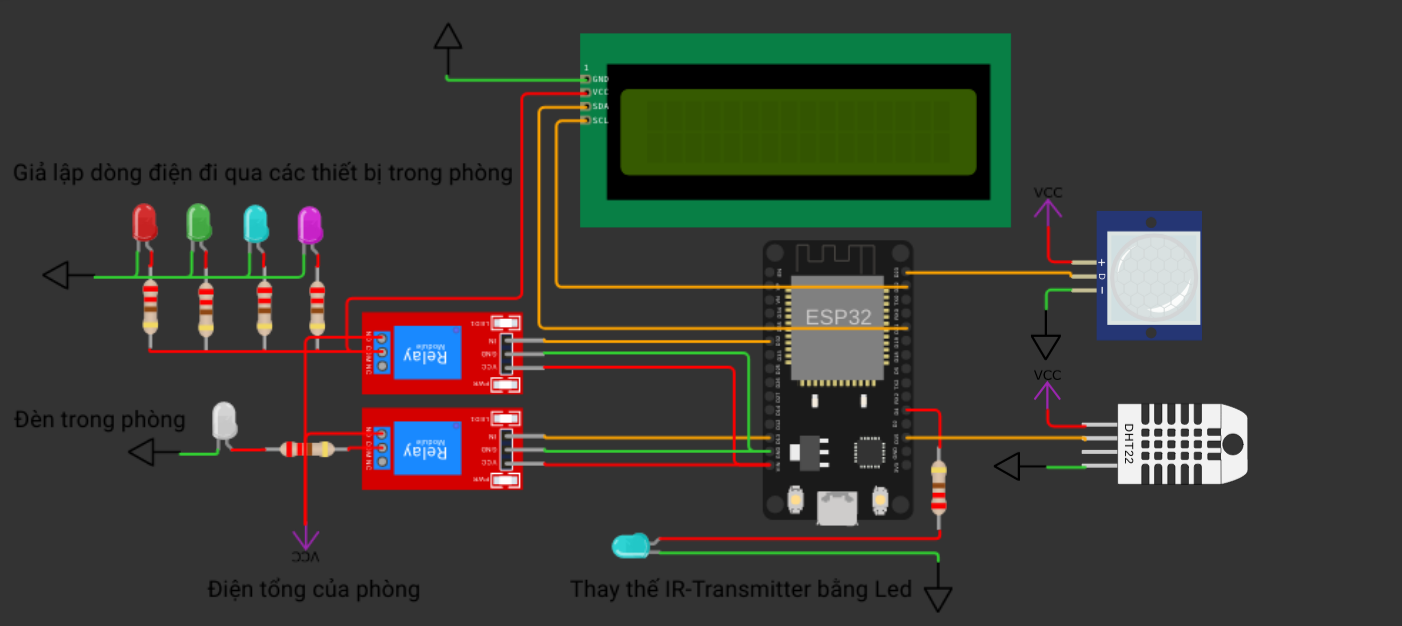
\includegraphics[width=\textwidth, keepaspectratio]{img/thiet_bi.png}
    \caption{Giả lập thiết bị hỗ trợ sử dụng điện thông minh trong phòng}
\end{figure}


\subsubsection{Các thiết bị sử dụng chính}
Dựa trên yêu cầu và qui định của đồ án cuối kì thì nhóm đã kết hợp các thiết bị cho sản phẩm ở hình trên như sau:
    \begin{itemize}
        \item Output: LCD, relay, IR-Transmitter
        \item Input: DHT22, cảm biến chuyển động (dạng hồng ngoại PIR).
        \item Board ESP32 có kết nối wifi.
    \end{itemize}

\subsubsection{Các thiết bị khác trong hình ảnh của sản phẩm}
\begin{itemize}
    \item Như đã được chú thích trong hình, vì không thể giả lập thiết bị IR-Transmitter nên nhóm đã sử dụng 1 bóng đèn led màu xanh dương (được nối trực tiếp với board ESP32). Khi bóng đèn led này chớp tắt tức là thiệt bị đã gửi tín hiệu hồng ngoại tới các thiết bị trong phòng.

    \item Bóng đèn led màu trắng chính là đèn chính trong phòng.

    \item 4 bóng đèn led còn lại được dùng để tương trưng cho các thiệt bị trong phòng đang có dòng điện đi qua. Nếu có điện trong phòng, 4 bóng đèn led này sẽ phát sáng tượng trưng cho việc các thiết bị điện trong phòng đang có điện.
\end{itemize}

\subsubsection{Tổng quát cách thức hoạt động của sản phẩm}
\begin{itemize}
    \item Sản phẩm này của nhóm sẽ nhận biết rằng người trong phòng hay không để thực hiện mở các thiết bị điện cần thiết. Thêm vào đó người dùng có thể kiểm soát được 2 chế độ "hoạt động" và "bảo vệ", trong đó: chế độ \textbf{"hoạt động"} sẽ giúp người dùng bật tắt thiết bị điện khi người dùng ra hay vào phòng, và chế độ \textbf{"bảo vệ"} sẽ ngắt cung cấp điện cho các thiết bị đồng thời cảnh báo người dùng khi có người vào phòng.

    \item Ngay khi khởi tạo, thiết bị \textbf{ESP32} sẽ thực hiện kết nối wifi, nếu việc kết nối có vấn đề sẽ tiếp tục thực hiện kết nối \textbf{trong vòng 5 phút}. Nếu sau 5 phút không kết nối được thì các chức năng xem thông tin trên \textbf{trang web hay điện thoại} sẽ không thể sử dụng, và để thưc hiện kết nối lại wifi sẽ thực hiện lại \textbf{sau 5 phút từ khi việc kết nối cuối cùng thất bại}.

    \item Trong trường hợp kết nối được wifi thì \textbf{ESP32} sẽ tiến hành kết nối \textbf{MQTT server} và \textbf{cloud server (Thingspeak)}. Việc cố gắng thực hiện kết nối giữa 2 server cũng sẽ diễn ra trong 5 phút và sẽ thực hiện kết nối lại cũng sau 5 phút kể từ lần cuối kết nối thất bại trong trường hợp đã kết nối wifi.
    
    \item Ngay sau khi các kết nối thành công, thiết bị sẽ mặc định được cài đặt chế độ \textbf{"hoạt động"}.
    \begin{figure}[!h]
        \centering
        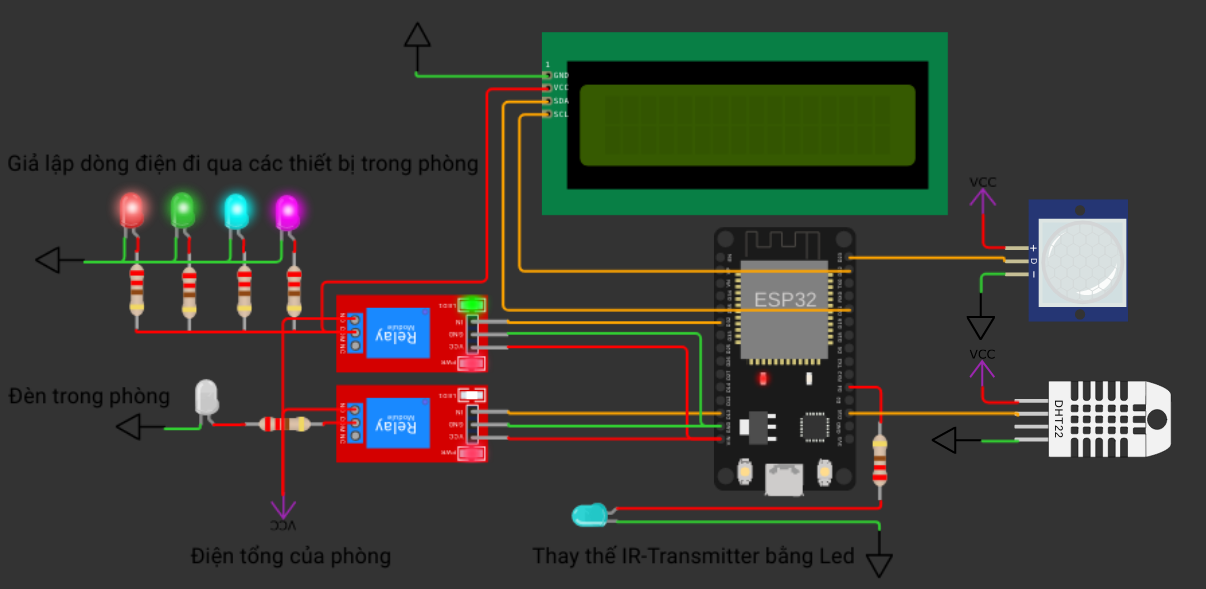
\includegraphics[width=\textwidth, keepaspectratio]{img/Khoi_tao.png}
        \caption{khi các kết nối thành công sẽ khởi tạo chế độ "hoạt động". 4 đèn led sáng tức là các thiết bị điện trong phòng đang được cung cấp điện}
    \end{figure}

    \pagebreak
    \item Khi có người bước vào phòng, \textbf{cảm biến chuyển động} sẽ nhận tín hiệu hồng ngoại và đèn trong phòng sẽ sáng, đồng thời trên màn hình \textbf{LCD} sẽ hiện lên thông tin về nhiệt độ, độ ẩm trong phòng.

    \begin{figure}[!h]
        \centering
        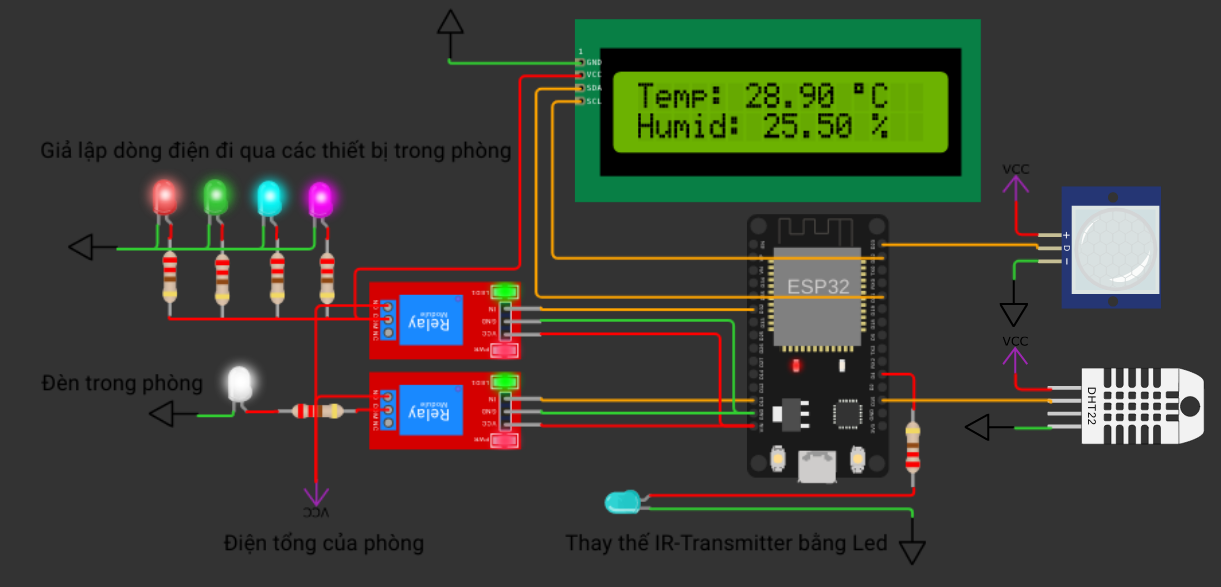
\includegraphics[width=\textwidth, keepaspectratio]{img/vao_phong.png}
        \caption{Đèn trong phòng sáng và thông tin được hiện trên màn hình LCD}
    \end{figure}

    \pagebreak
    \item Ngoài ra khi người dùng trong phòng và nhiệt độ lớn hơn 30°C thì máy lạnh sẽ được tự động mở thông qua thiết bị \textbf{IR-Transmitter}.

    \begin{figure}[!h]
        \centering
        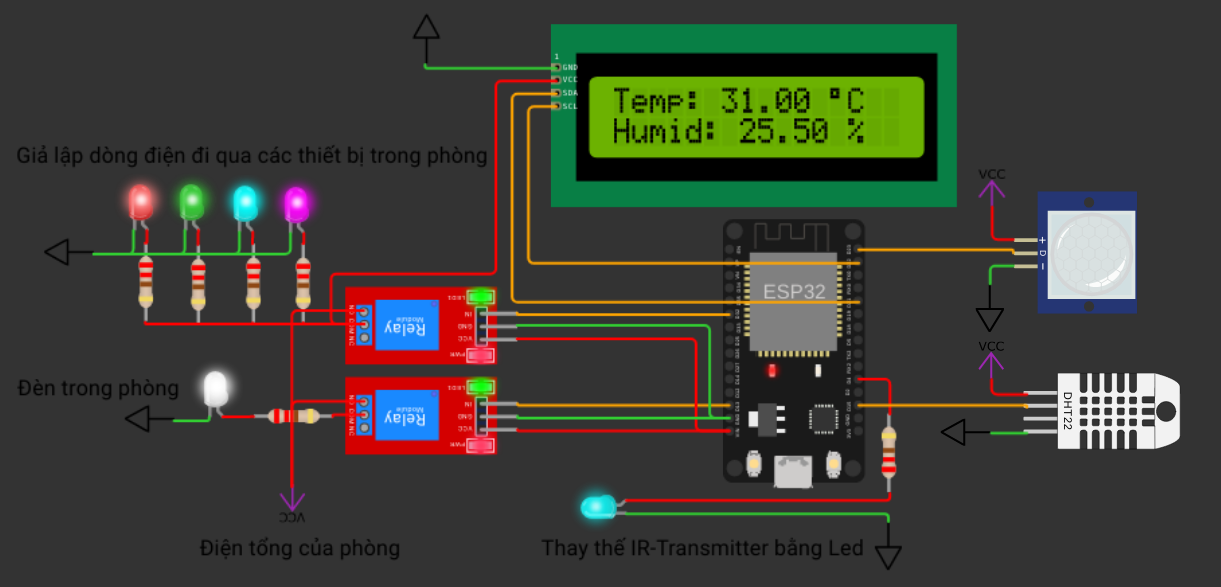
\includegraphics[width=\textwidth, keepaspectratio]{img/mlanh_mo.png}
        \caption{Đèn led màu xanh đại diện cho IR-Transmitter sáng tức là đã phát tín hiệu hồng ngoại}
    \end{figure}

    \item Sau khi không còn ai trong phòng thì các thiết bị sẽ được tắt sau 1 khoảng thời gian nhất định, cụ thể  \textbf{máy lạnh} sẽ được tắt sau khoảng 30 phút tính từ thời điểm không có người nào trong phòng, còn \textbf{các thiết bị khác} sẽ tắt sau khoảng 2 phút.

    \item Đối với trường hợp \textbf{"Bảo vệ"}, các thiết bị trong phòng sẽ không được cung cấp nguồn điện, và khi có người vào trong phòng, sản phẩm sẽ cảnh báo về \textbf{chat bot telegram} rằng có người vào phòng.
    \begin{figure}[H]
        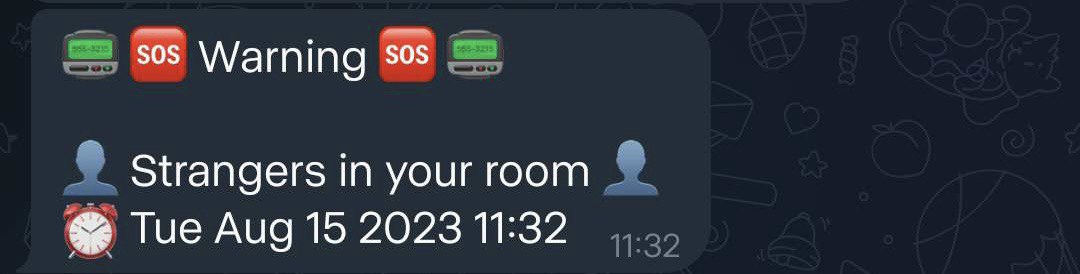
\includegraphics[width=\textwidth, keepaspectratio]{img/warning.jpg}
        \centering
        \caption{Tin nhắn cảnh báo từ chat bot telegram}
    \end{figure}
    

    \item Ngoài ra, nhóm đã thiết lập cho phép thay đổi 2 chế độ này thông qua các lệnh được cài đặt trong khung chat bot của telegram, giúp người dùng có thể thay đổi nhanh chóng. Lệnh để  chuyển đổi sang chế độ \textbf{"hoạt động"} là \textbf{"/workingmode"} và chuyển sang chế độ \textbf{"bảo vệ"} là \textbf{"/safetymode"}.
    \begin{figure}[H]
        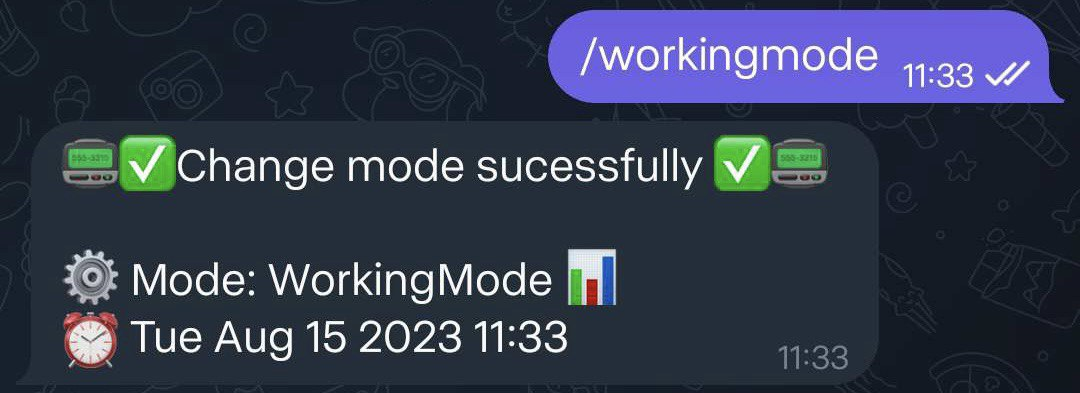
\includegraphics[width=\textwidth, keepaspectratio]{img/change_work.jpg}
        \centering
        \caption{Lệnh chuyển đổi sang chế độ "hoạt động"}
    \end{figure}

    \begin{figure}[H]
        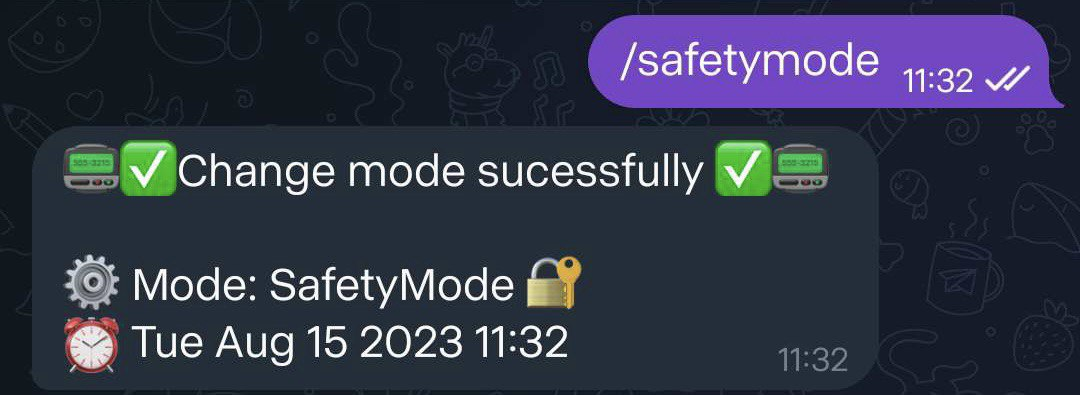
\includegraphics[width=\textwidth, keepaspectratio]{img/change_safe.jpg}
        \centering
        \caption{Lệnh chuyển đổi sang chế độ "bảo vệ"}
    \end{figure}
    
    \item Thêm vào đó, người dùng có thể xem thông tin về nhiệt độ, độ ẩm, chuyển đổi chế độ trên \textbf{trang web} và cũng như lịch sử của các thông tin nhờ việc \textbf{lưu và lấy dữ liệu từ cloud}.
    
    \begin{figure}[H]
        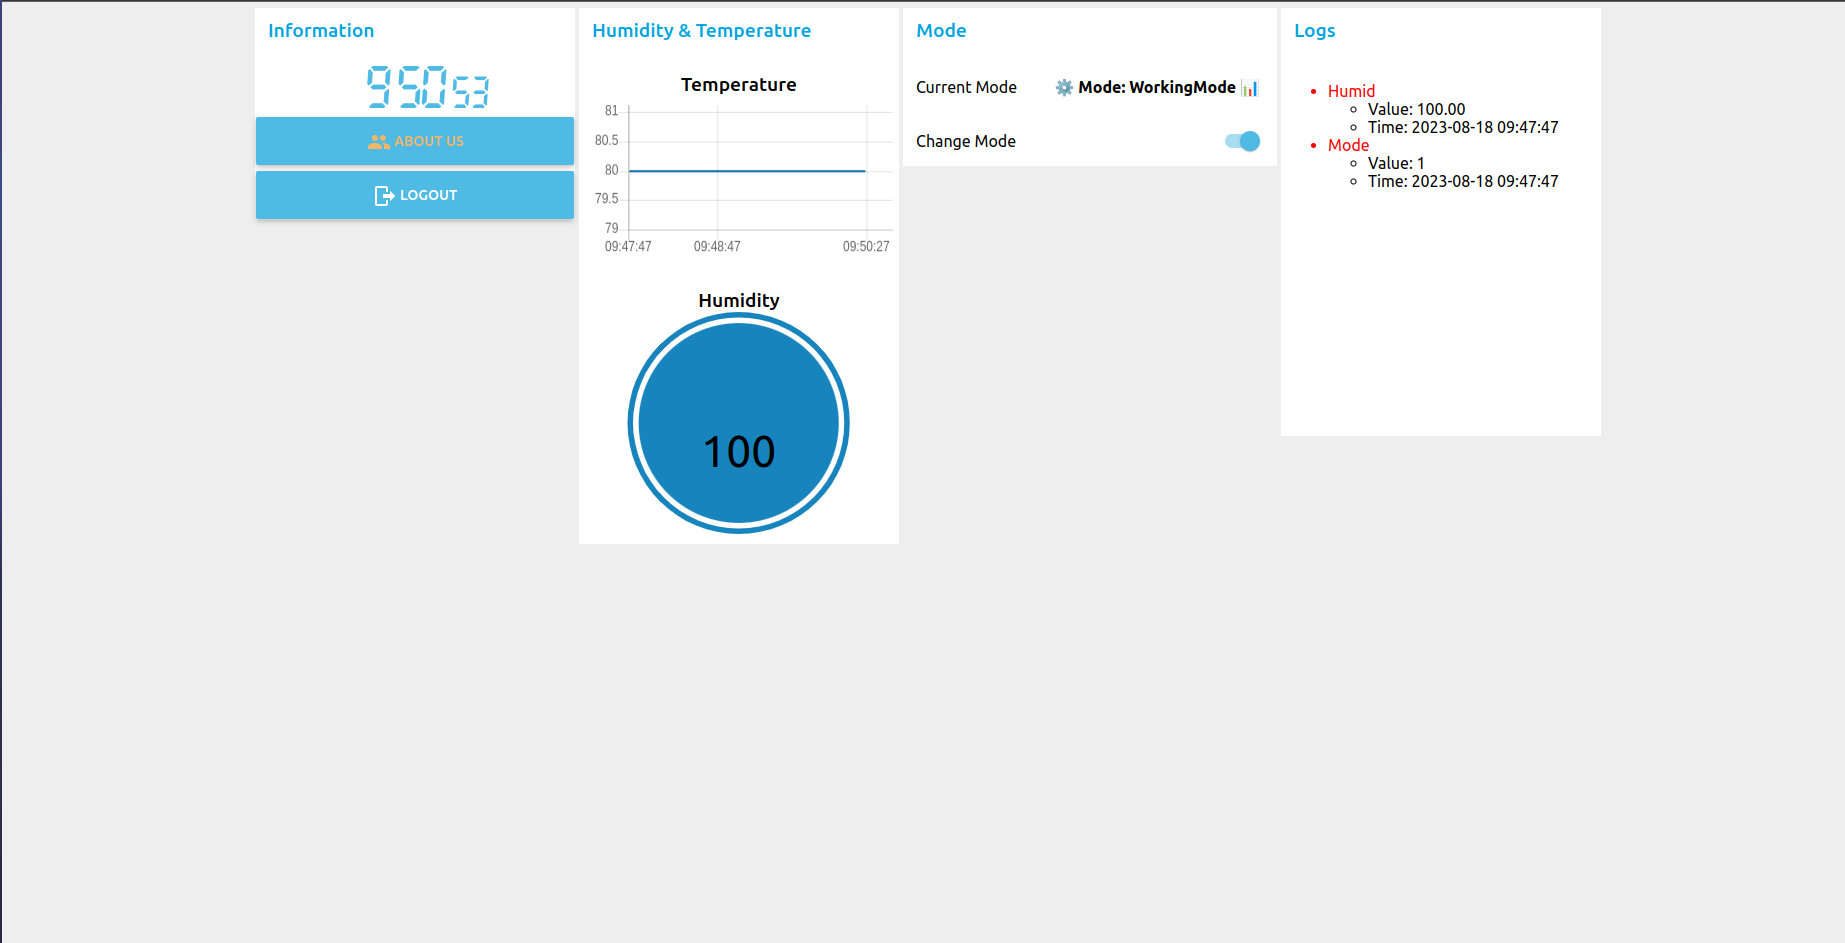
\includegraphics[width=\textwidth, keepaspectratio]{img/web_UI.png}
        \centering
        \caption{Hình ảnh tổng quát về trang web}
    \end{figure}
\end{itemize}


\subsection{Sơ đồ truyền và nhận dữ liệu của các thiết bị IOT và server}
\begin{figure}[!h]
    \centering
    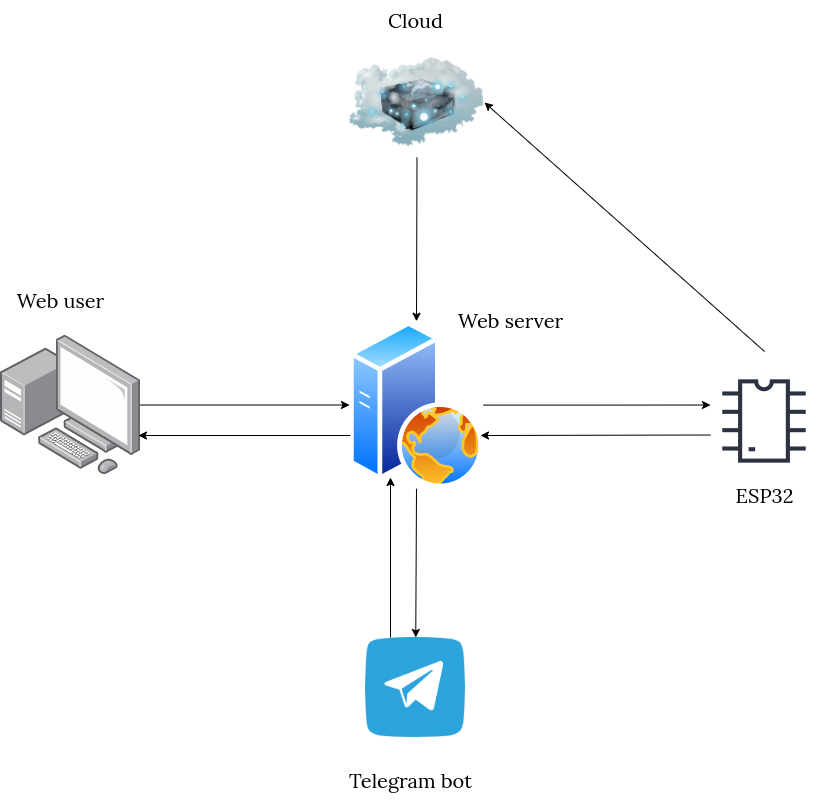
\includegraphics[width=\textwidth, height=0.4\textheight, keepaspectratio]{img/Diagram.png}
    \caption{Sơ đồ  truyền nhận dữ liệu}
\end{figure}

\newpage
\subsection{Thiết kế 3D sản phẩm của nhóm}
Dưới đây sẽ là chi tiết về hình ảnh của sản phẩm được thiết kế 3D ở nhiều góc độ.
\begin{itemize}
    \item Đầu tiên phải nói tới vị trí đặt thiết bị ở trong phòng. Nhóm đã thiết kế bố trí sản phẩm ngay phía bên trái của cửa phòng để có thể nhận diện nhanh nhất khi có người vào phòng.
    \begin{figure}[!h]
        \centering
        \includegraphics[width=0.5\textwidth, height=0.4\textheight, keepaspectratio]{img/PhoiCanh-01.png}
        \caption{Vị trí đặt thiết bị ở trong phòng}
    \end{figure}

    \item Đến với chi tiết của sản phẩm, trước hết các thiết bị của sản phẩm được liên kết với nhau và đặt trong hộp làm bằng hộp nhựa acrylic. Bên ngoài của hộp là 2 thiết bị \textbf{Cảm biến chuyển động} và \textbf{màn hình LCD} để người dùng dễ dàng nhìn thấy thông số trong phòng và giúp thiết bị cảm nhận người trong phòng tốt nhất.
    \begin{figure}[!ht]
        \centering
        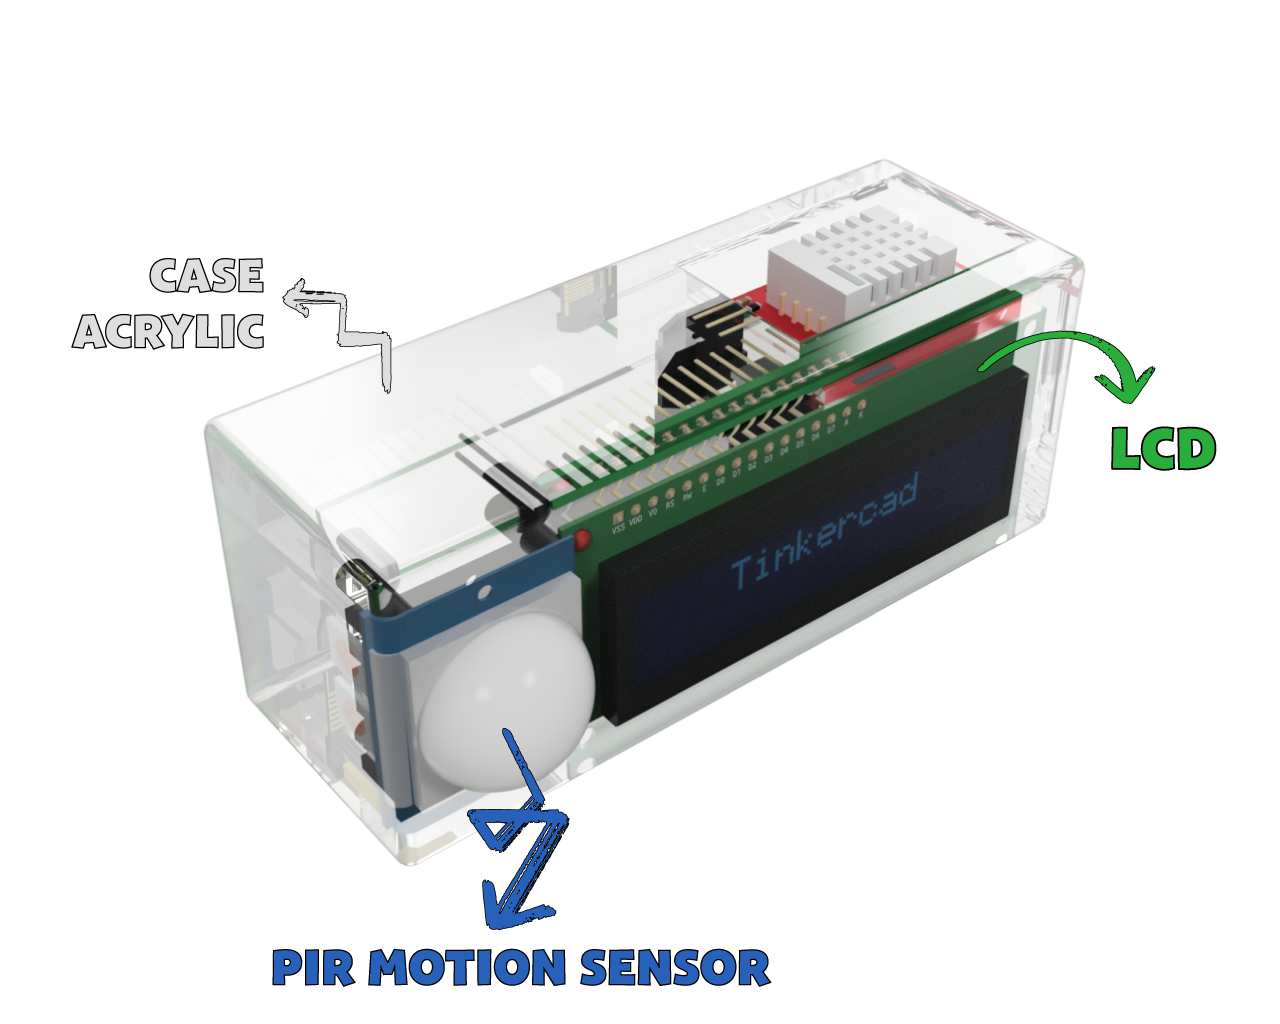
\includegraphics[width=0.5\textwidth, keepaspectratio]{img/1-01.png}
        \caption{Mặt trước của sản phẩm}
    \end{figure}
    \pagebreak
    \item Phía trên của sản phẩm chính là thiết bị \textbf{DHT22} dùng để  đo nhiệt độ, độ ẩm. Thiết bị này sẽ kết nối với \textbf{LCD} và thông tin nhiệt độ, độ ẩm sẽ in ra màn hình.
    \begin{figure}[!ht]
        \centering
        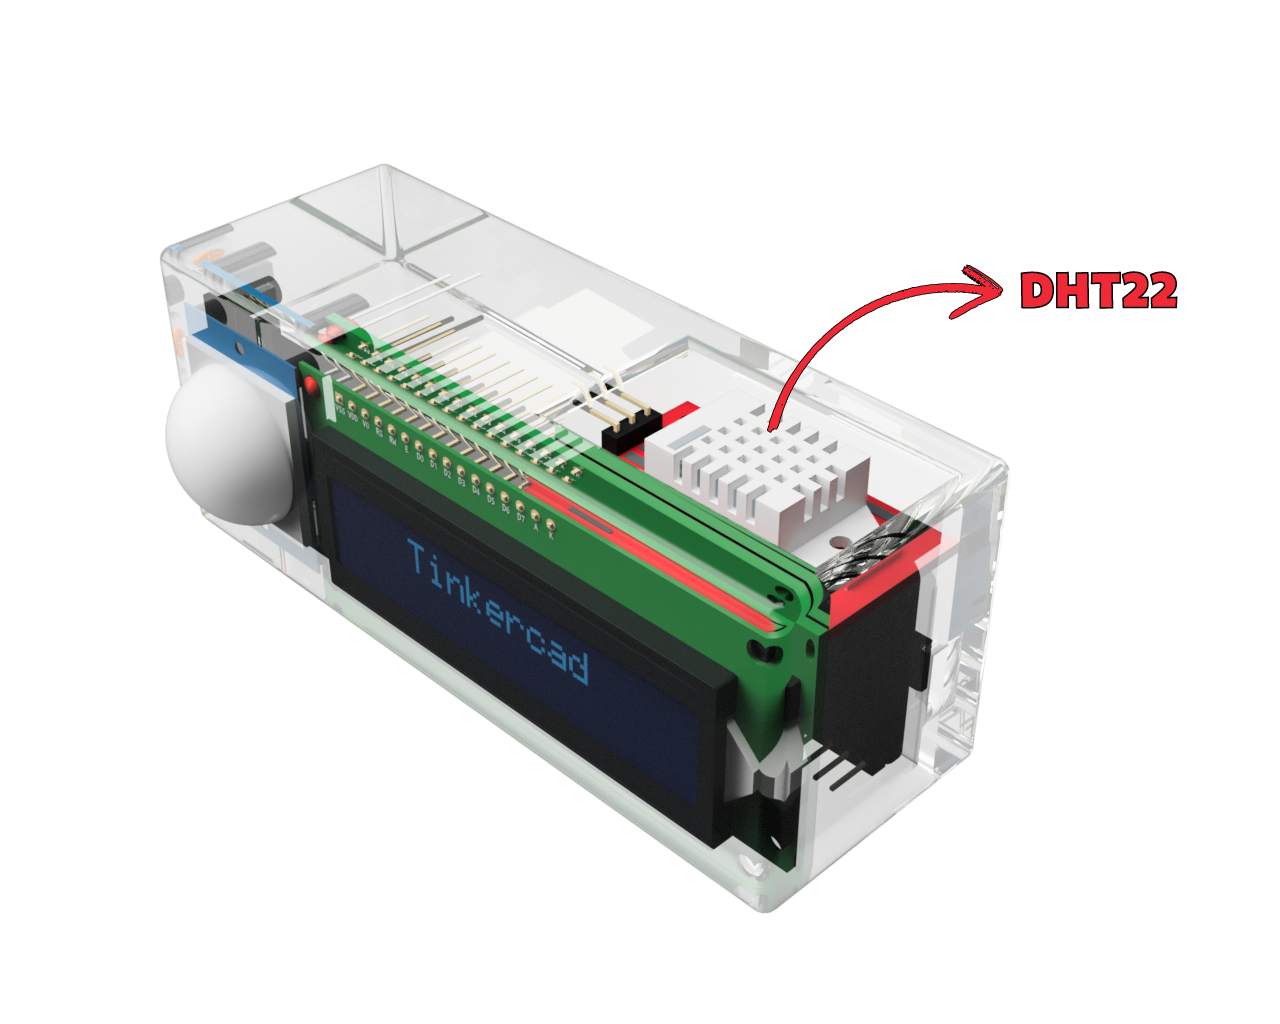
\includegraphics[width=0.5\textwidth, keepaspectratio]{img/2-01.png}
        \caption{Mặt trên của sản phẩm}
    \end{figure}

    \pagebreak
    \item Mặt sau của sản phẩm là thiết bị \textbf{ESP32} và vị trí giữa \textbf{ESP32} và \textbf{LCD} là thiết bị \textbf{Relay}.
    \begin{figure}[!ht]
        \centering
        \includegraphics[width=0.5\textwidth, keepaspectratio]{img/3-01.png}
        \caption{Mặt sau của sản phẩm}
    \end{figure}
    
    \item Cuối cùng nhìn từ mặt sau chúng ta còn thấy được chân của thiết bị  \textbf{IR-Transmitter}, phần đầu để phát tín hiệu hồng ngoại của thiết bị sẽ nằm phía mặt trước của sản phẩm.
    \begin{figure}[H]
        \includegraphics[width=0.5\textwidth, keepaspectratio]{img/4-01.png}
        \centering
        \caption{Vị trí của IR-Transmitter}
    \end{figure}

    
\end{itemize}

\newpage
\subsection{Giao diện và chức năng của web}
\begin{itemize}
    \item Đầu tiên ngay khi truy cập vào trang web thì sẽ là màn hình đăng nhập, yêu cầu người dùng nhập \textbf{tên đăng nhập ("admin") và mật khẩu ("admin")}.
    
    \begin{figure}[H]
        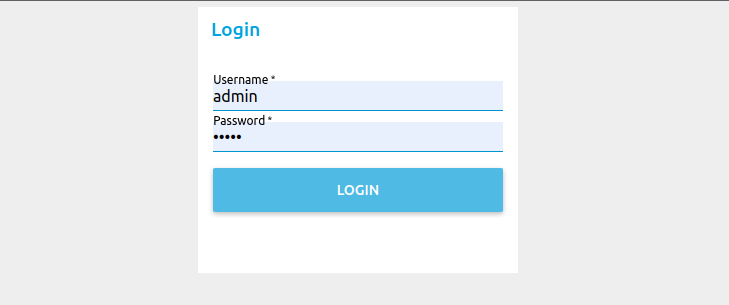
\includegraphics[width=\textwidth, keepaspectratio]{img/log_in_page.png}
        \centering
        \caption{Giao diện trang đăng nhập của website}
    \end{figure}
    
    \item Khi đăng nhập thành công, người dùng sẽ chuyển sang trang chính của website.
    \begin{figure}[H]
        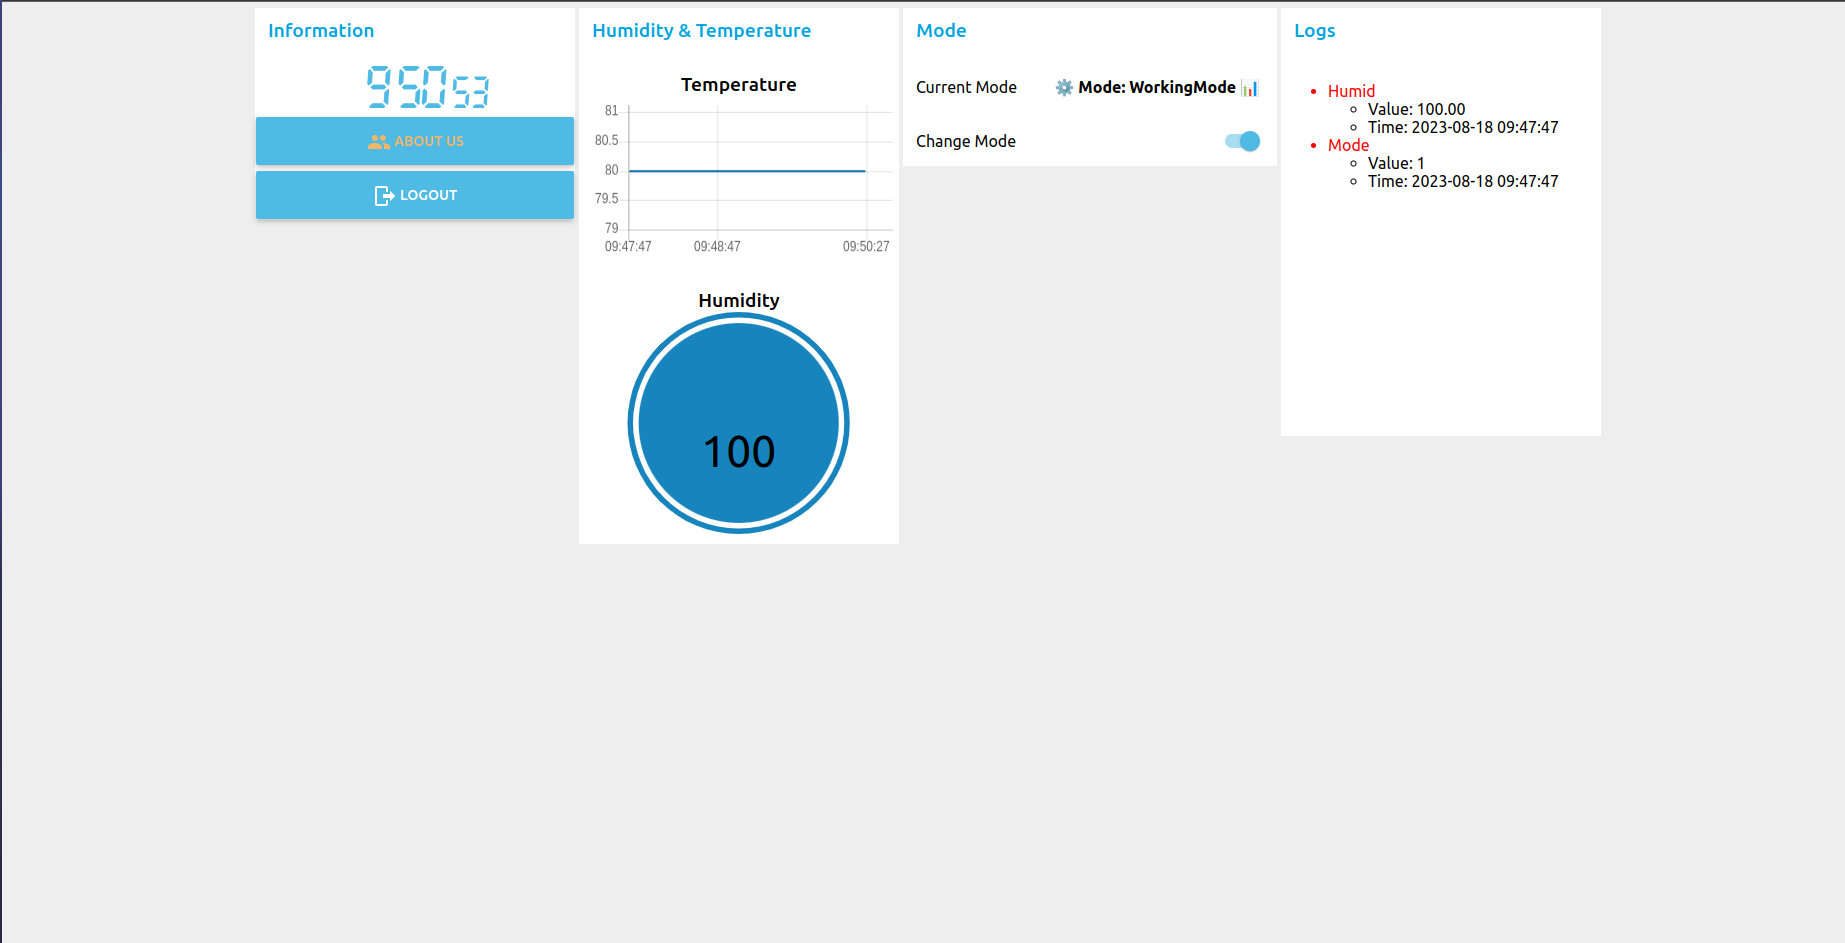
\includegraphics[width=\textwidth, keepaspectratio]{img/web_UI.png}
        \centering
        \caption{trang chính của website}
    \end{figure}

    \item Nhóm đã thiết kế ở trang chính của trang web này mỗi chức năng sẽ đươc đặt ở 1 khung riêng biết để người dùng dễ dàng nhận biết và sử dụng. Cụ thể như sau:
    
    \begin{itemize}
        \item Đầu tiên ở bên trái ngoài cùng của trang web là khung để hiển thị \textbf{thời gian, nút chuyển tới thông tin của nhóm và nút đăng xuất khỏi trang web}.
        \begin{figure}[H]
            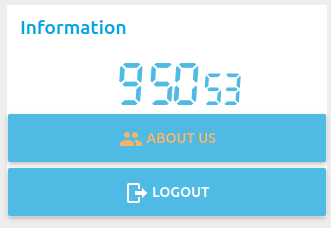
\includegraphics[width=\textwidth, keepaspectratio]{img/information_group.png}
            \centering
            \caption{Khung hiển thị thời gian, thông tin nhóm và nút đăng xuất}
        \end{figure}
        Ở trang \textbf{ABOUT US} sẽ hiển thị \textit{Tên, mã số sinh viên, vai trò, và đường dẫn đến email} của mỗi thành viên.
        \begin{figure}[H]
            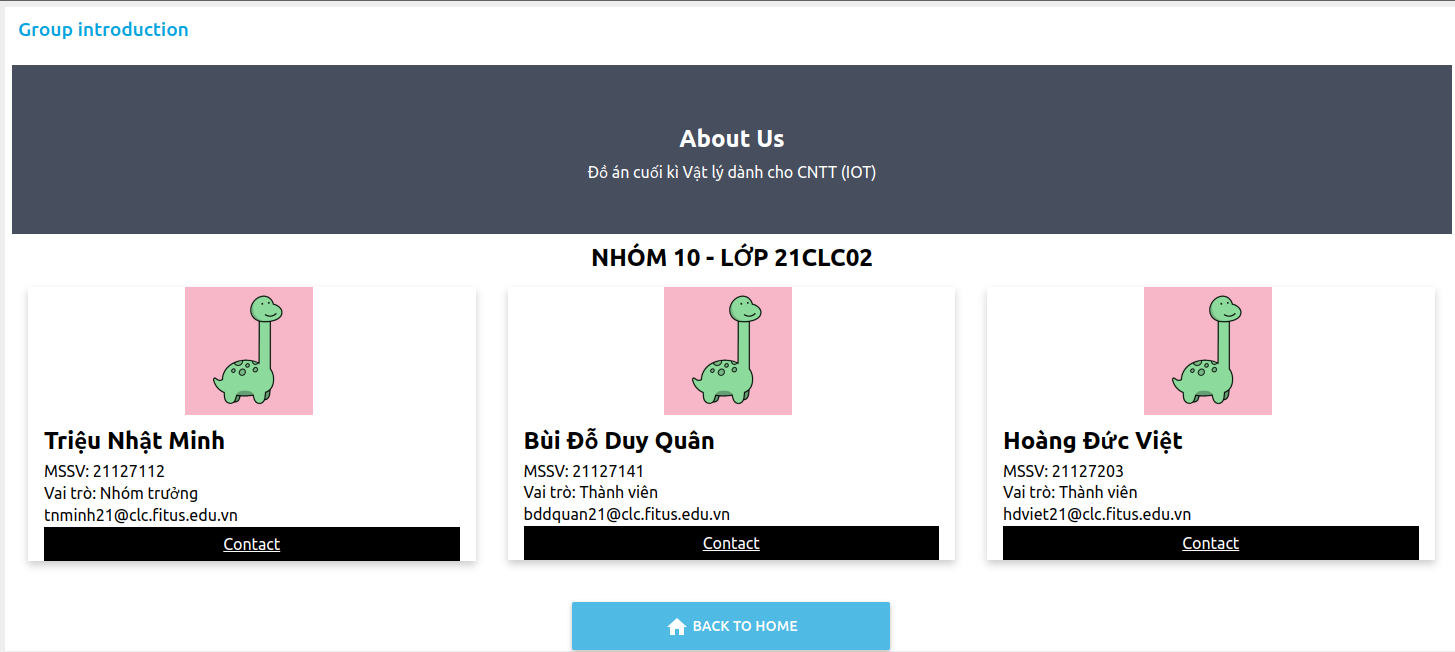
\includegraphics[width=\textwidth, keepaspectratio]{img/about_us.png}
            \centering
            \caption{Thông tin của nhóm}
        \end{figure}

        \item Khung tiếp theo sẽ hiển thị biểu đồ đường về \textbf{nhiệt độ} và biểu đồ tròn về \textbf{độ ẩm} ở thời điểm hiện tại.
        \begin{figure}[H]
            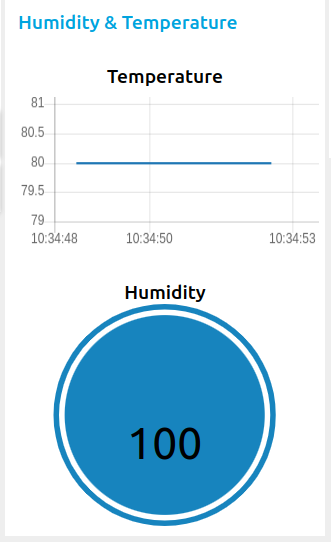
\includegraphics[width=\textwidth, height=0.4\textheight, keepaspectratio]{img/temp_humid.png}
            \centering
            \caption{Biểu đồ nhiệt độ và độ ẩm}
        \end{figure}

        \item Kế tiếp chính là khung \textbf{hiển thị chế độ hiện tại và nút thay đổi chế độ}. Với \textbf{nút thay đổi chế độ}, người dùng có thể thay đổi chế độ "hoạt động" hay "bảo vệ" của thiết bị ở trong phòng.

        \begin{figure}[H]
            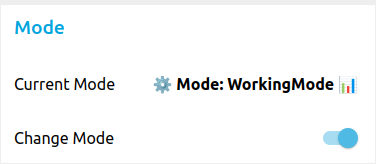
\includegraphics[width=\textwidth, keepaspectratio]{img/mode.png}
            \centering
            \caption{Thông tin và chức năng chuyển chế độ}
        \end{figure}
        
        \item Cuối cùng là khung \textbf{logs} để hiển thị lịch sử của những lần thay đổi chế độ và các thông tin về nhiệt độ, độ ẩm trong phòng.
        
        \begin{figure}[H]
            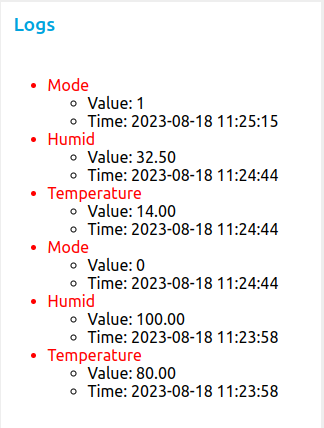
\includegraphics[width=\textwidth, height=0.4\textheight, keepaspectratio]{img/logs.png}
            \centering
            \caption{Lịch sử các thông tin}
        \end{figure}
    \end{itemize}
\end{itemize}

\newpage
\subsection{Xây dựng flow trong NodeRed}
Giao diện và chức năng của web được xây dựng bằng NodeRed qua việc kết hợp các node chức năng để  tạo thành flow cho trang web.


\begin{enumerate}
    \item Đầu tiên chính là phần node cho \textbf{đăng nhập vào trang web}. Node này sẽ có chức năng kiểm tra tài khoản và mật khẩu của người dùng, nếu đúng thì sẽ cho phép người dùng đăng nhập vào trang web, nếu sai thì sẽ hiện thông báo lỗi.
    \begin{figure}[H]
        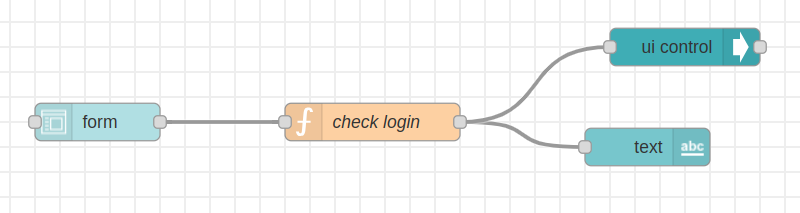
\includegraphics[width=\textwidth, keepaspectratio]{img/flow/login_node.png}
        \centering
        \caption{Các node về đăng nhập tài khoản}
    \end{figure}
    Sau khi người dùng điền tên đăng nhập và mật khẩu vào \textbf{form} thì hàm \textbf{check login} sẽ kiểm tra thông tin đăng nhập có hợp lệ hay không. Nhóm đã thống nhất rằng tên đăng nhập và mật khẩu để vào web đều là \textbf{"admin"}. Đăng nhập thành công thì sẽ chuyển sang màn hình chính cùa web, và ngược lại thì sẽ đưa ra dòng thông báo đăng nhấp thất bại.
    \begin{figure}[H]
        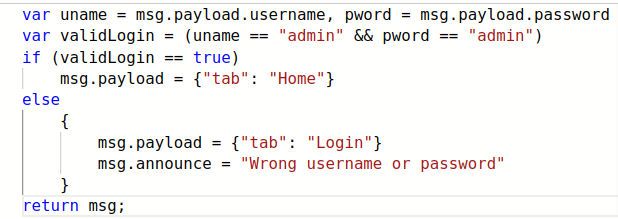
\includegraphics[width=\textwidth, keepaspectratio]{img/flow/check_login.png}
        \centering
        \caption{Hàm kiểm tra tài khoản và mật khẩu}
    \end{figure}

    \item Tiếp đó là các node cho giao diện về \textbf{đồng hồ và chức năng đăng xuất}. Để có thể lấy thông tin giờ/phút/giây hiện tại thì sẽ sử dụng node \textbf{digital clock} và 1 node \textbf{inject} để liên tục lấy thông tin thời gian liên tực sau 1 giây và hiển thị lên màn hình trang web.
    \begin{figure}[H]
        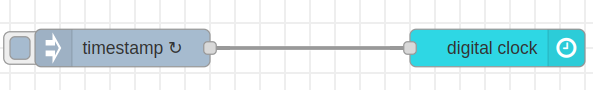
\includegraphics[width=\textwidth, keepaspectratio]{img/flow/clock.png}
        \centering
        \caption{Node về đồng hồ} 
    \end{figure}
    Nút \textbf{Log out} trên màn hình sẽ hỗ trợ chức năng thoát khỏi trang chính của web và quay trở lại trang đăng nhập trước đó.
    \begin{figure}[H]
        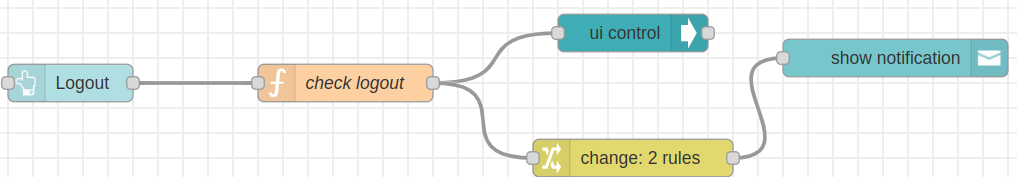
\includegraphics[width=\textwidth, keepaspectratio]{img/flow/logout.png}
        \centering
        \caption{Node về đăng xuất}
    \end{figure}

    \item Kế đến đó chính là các node hỗ trợ chức năng chính của trang web. Đầu tiên để  hiển thị thông tin nhiệt độ, độ ẩm trong phòng thì nhóm đã sử dụng node \textbf{MQTT in}-là node sử dụng giao thức \textbf{MQTT}. Node này được cài đặt sẽ kết nối với server \textbf{broker.emqx.io} thông qua giao thức MQTT và lấy thông tin được đưa lên về nhiệt độ, độ ẩm từ thiết bị \textbf{ESP32} và hiển thị lên trang web.
    \begin{figure}[H]
        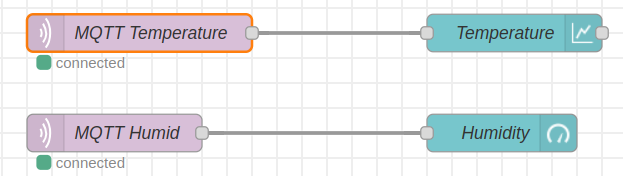
\includegraphics[width=\textwidth, keepaspectratio]{img/flow/mqtt_in.png}
        \centering
        \caption{Node lấy thông tin nhiệt độ, độ ẩm}
    \end{figure}

    \begin{figure}[H]
        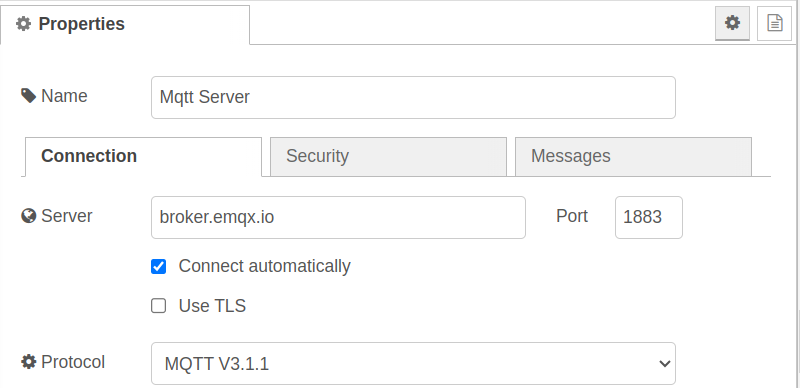
\includegraphics[width=\textwidth, keepaspectratio]{img/flow/configure_mqtt.png}
        \centering
        \caption{Thiết lập cho node MQTT in}
    \end{figure}
    
    \item Phần hiển thị thông tin đang ở chế độ nào cũng sẽ được thực hiện bằng cách lấy thông tin chế độ từ server đã được gửi từ \textbf{ESP32}. Hình ảnh giao diện về chế độ sẽ được cập nhật trên màn hình web theo đúng với thông tin chế độ của thiết bị. Đồng thời sản phẩm còn cho phép gửi thông tin chế độ và thời gian đã chuyển sang chế độ đó vào khung chat bot của telegram.
    Nhóm đã sử dụng node \textbf{sender} của \textbf{telegram bot} giúp truyền thông tin về chat box với bot của người dùng. Node này sẽ được khởi tạo bởi một mã token được cấp bởi \textbf{telegram bot father} và thông tin sẽ được gửi vào khung chat box của bot có mã token đó.
    \begin{figure}[H]
        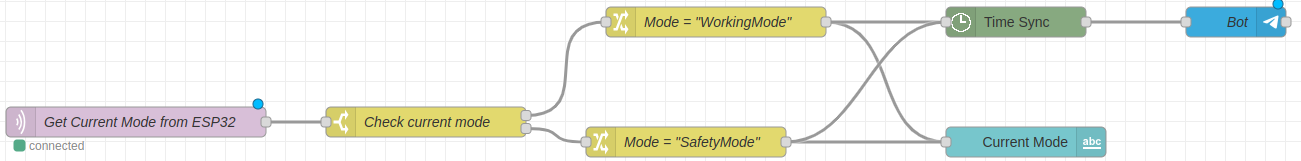
\includegraphics[width=\textwidth, keepaspectratio]{img/flow/send_current_mode.png}
        \centering
        \caption{Node gửi thông tin chế độ}
    \end{figure}

    \begin{figure}[H]
        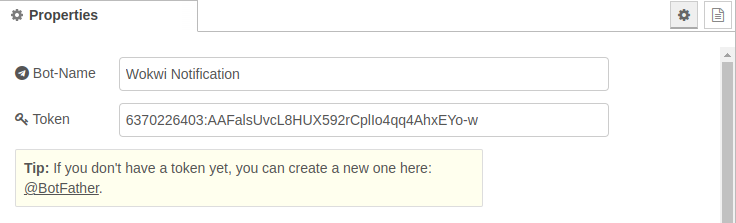
\includegraphics[width=\textwidth, keepaspectratio]{img/flow/configure_bot.png}
        \centering
        \caption{Thiết lập cho node sender}
    \end{figure}

    \item 1 chức năng cũng được cài đặt khá tương tự với chức năng trên đó là \textbf{gửi tin nhắn cảnh báo về người dùng}. Điểm tương đồng là cũng sẽ sử dụng node \textbf{MQTT in} để lấy dữ liệu khi có người vào phòng và cũng sẽ tạo tin nhắn và gửi qua chat box của \textbf{bot telegram}.
    \begin{figure}[H]
        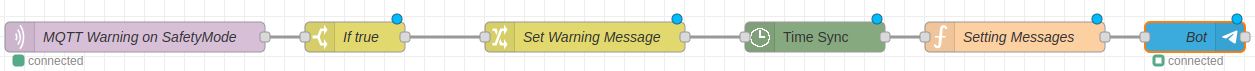
\includegraphics[width=\textwidth, keepaspectratio]{img/flow/send_warning.png}
        \centering
        \caption{Node gửi tin nhắn cảnh báo}
    \end{figure}

    \item Chức năng tiếp theo được đề cập đến chính là \textbf{Chuyển đổi chế độ}. Nhóm đã thiết kế để cho người dùng có thể điều chỉnh giữa 2 chế độ thông qua 2 cách đó chính là \textbf{trên web và qua bot telegram}. \textbf{Nút bấm chuyển đổi} được cài đặt để khi chuyển sang chế độ nào sẽ gửi thông tin về lên server thông qua \textbf{MQTT out} và thông tin đó sẽ chuyển về \textbf{ESP32} để điều khiển các thiết bị trong phòng.
    \begin{figure}[H]
        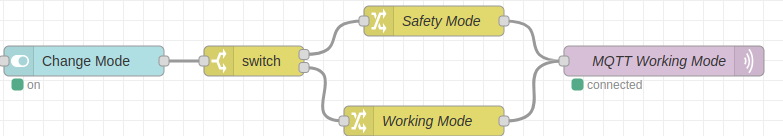
\includegraphics[width=\textwidth, keepaspectratio]{img/flow/change_btn_mode.png}
        \centering
        \caption{Node chuyển đổi chế độ}
    \end{figure}
    Việc gửi lệnh chuyển đổi thông qua \textbf{bot telegram} thì sẽ sử dụng node \textbf{telegram receiver} để nhận lệnh từ khung chat box của bot. Thông tin lệnh được gửi tới sẽ dược kiểm tra xem có phải là loại \textbf{message} hay không và nội dung phải là 1 trong 2 câu lệnh \textbf{safetymode} và \textbf{workingmode} thì mới được lưu lại để \textbf{nút chuyển đổi} cũng nhận thông tin và gửi lên server.
    \begin{figure}[H]
        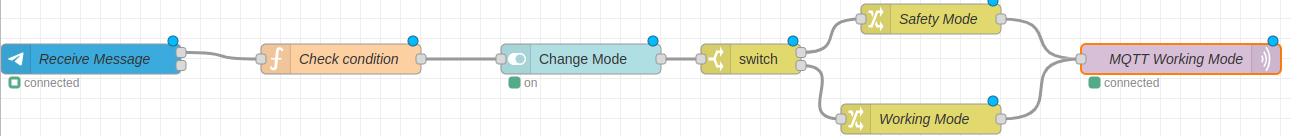
\includegraphics[width=\textwidth, keepaspectratio]{img/flow/bot_receiver.png}
        \centering
        \caption{Node nhận lệnh chuyển đổi chế độ}
    \end{figure}

    \begin{figure}[H]
        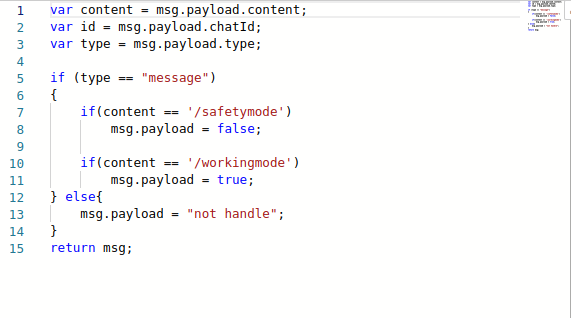
\includegraphics[width=\textwidth, keepaspectratio]{img/flow/check_message.png}
        \centering
        \caption{Hàm kiểm tra lệnh chuyển đổi chế độ}
    \end{figure}
    
    \item Cuối cùng là chức năng lấy dữ liệu từ trên cloud \textbf{thingspeak} về. Node mà nhóm đã sử dụng chính là \textbf{https request} để thực hiện yêu cầu tới đường dẫn \textbf{API key} của \textbf{thingspeak} để lấy thông số của gần nhất của 3 thông tin \textbf{nhiệt độ, độ ẩm và chế độ và thời điểm} của các thông số đó. Nút \textbf{inject} sẽ có nhiệm vụ khởi động \textbf{request} liên tục sau 1 giây và khi phía cloud có sự thay đổi thông số của bất kì thông tin nào thì thông số đó sẽ được cập nhật lên trang web thông qua hàm \textbf{control log list}. Hàm này sẽ có nhiệm vụ thực hiện thông số mới nhất và khi liên tục nhận dữ liệu từ cloud, hàm sẽ tiến hành kiểm tra xem thông số mới nhận được có thay đổi hay không, nếu thay đổi thì sẽ đẩy lên hàng đầu của \textbf{log list} và in ra màn hình web, nếu không thay đổi thì sẽ không cập nhật để tránh tình trạng đưa lên các thông số chưa thay đổi. Chú ý rằng \textbf{API key} được lấy sẽ thêm tham số truy vấn \textbf{timezone} để chuyển múi giờ về \textbf{GMT+7} (chi tiết như ở \href{https://www.mathworks.com/help/thingspeak/readdata.html}{đây}).
    \begin{figure}[H]
        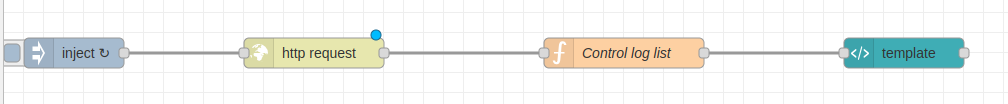
\includegraphics[width=\textwidth, keepaspectratio]{img/flow/get_data.png}
        \centering
        \caption{Node lấy dữ liệu từ cloud}
    \end{figure}

    \begin{figure}[H]
        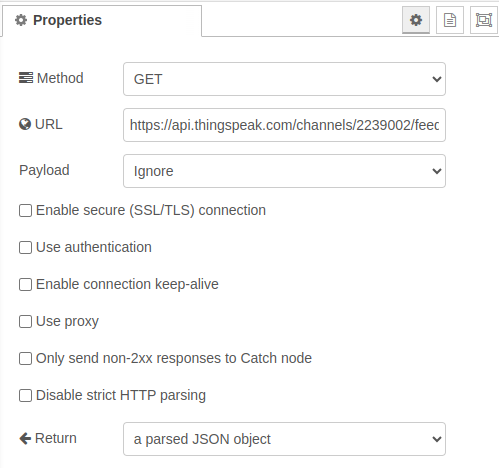
\includegraphics[width=\textwidth, height=0.5\textheight, keepaspectratio]{img/flow/configure_request.png}
        \centering
        \caption{Thiết lập cho node https request}
    \end{figure}

    với giá trị \textbf{URL: \url{https://api.thingspeak.com/channels/2239002/feeds.json?api_key=20EMGP6E0ZMPG8N1&results=1&timezone=Asia\%2FJakarta}}
    \pagebreak
    \begin{lstlisting}[language=JavaScript, caption={function of control log list}]
        var logList = flow.get("logList")
        var topic1 = "", payload1 = ""
        var topic2 = "", payload2 = ""
        var topic3 = "", payload3 = ""

        var time = msg.payload.feeds[0].created_at
        time = time.replace("T", " ")
        time = time.replace("+07:00", "")

        if (msg.payload.feeds[0].field1 != flow.get("prevMode"))
        {
            topic1 = "Mode"
            payload1 = msg.payload.feeds[0].field1
            flow.set("prevMode", payload1)
        }

        if (msg.payload.feeds[0].field2 != flow.get("prevTemperature")) 
        {
            topic2 = "Temperature"
            payload2 = msg.payload.feeds[0].field2
            flow.set("prevTemperature", payload2)
        }

        if (msg.payload.feeds[0].field3 != flow.get("prevHumid")) 
        {
            topic3 = "Humid"
            payload3 = msg.payload.feeds[0].field3
            flow.set("prevHumid", payload3)
        }

        if (topic1 != "")
        {
            msg = {}
            msg.topic = topic1
            msg.payload = payload1
            msg.time = time
            logList.unshift(msg)
        }

        if (topic2 != "") 
        {
            msg = {}
            msg.topic = topic2
            msg.payload = payload2
            msg.time = time
            logList.unshift(msg)
        }

        if (topic3 != "") 
        {
            msg = {}
            msg.topic = topic3
            msg.payload = payload3
            msg.time = time
            logList.unshift(msg)
        }

        if (logList.length > 10) 
        {
            logList.shift();
            logList.length = 10;
        }

        flow.set("logList", logList)
        msg = {}
        msg.payload = logList
        return msg;
    \end{lstlisting}

    Ngoài ra để  giúp in các thông tin được đồng nhất thì nhóm đã thiết kế  hàm để kiểm soát thông số  khởi tạo. Nếu trên cloud đang có thông số sẵn thì sẽ lấy thông số mới nhất của từng thông tin, và nếu chưa thì sẽ khởi tạo cho các thông số của thông tin giá trị cực nhỏ để khi bắt đầu chạy thiết bị thì sẽ lấy thông số  hiện tại mà sản phẩm thu nhận được.
    \begin{figure}[H]
        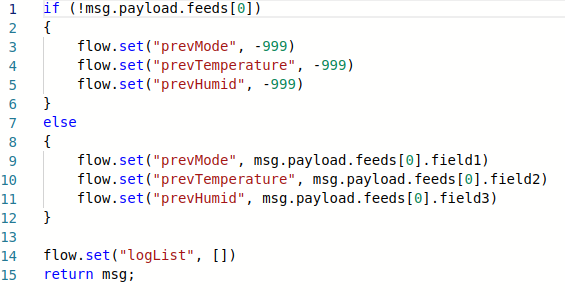
\includegraphics[width=\textwidth, keepaspectratio]{img/flow/init_log_value.png}
        \centering
        \caption{Hàm kiểm soát thông số khởi tạo}
    \end{figure}
\end{enumerate}
\pagebreak
\section{Phân công công việc}
\begin{table}[!h]
    \centering
    \resizebox{\textwidth}{!}{%
    \begin{tabular}{|c|l|c|}
    \hline
    \rowcolor[HTML]{DDD9C4} 
    \multicolumn{1}{|l|}{\cellcolor[HTML]{00D2CB}{\color[HTML]{FFFFFF} \textbf{}}} & {\color[HTML]{000000} \textbf{Công việc}} & {\color[HTML]{000000} \textbf{Người thực hiện}} \\ \hline
    \rowcolor[HTML]{F2DCDB} 
    \cellcolor[HTML]{E6B8B7} & Cài đặt lớp PIR & Đức Việt \\ \cline{2-3} 
    \rowcolor[HTML]{F2DCDB} 
    \cellcolor[HTML]{E6B8B7} & Cài đặt lớp DHT & Nhật Minh \\ \cline{2-3} 
    \rowcolor[HTML]{F2DCDB} 
    \cellcolor[HTML]{E6B8B7} & Cài đặt lớp IR & Đức Việt \\ \cline{2-3} 
    \rowcolor[HTML]{F2DCDB} 
    \cellcolor[HTML]{E6B8B7} & Cài đăt lớp LCD & Duy Quân \\ \cline{2-3} 
    \rowcolor[HTML]{F2DCDB} 
    \cellcolor[HTML]{E6B8B7} & Cài đặt lớp relay & Đức Việt \\ \cline{2-3} 
    \rowcolor[HTML]{F2DCDB} 
    \cellcolor[HTML]{E6B8B7} & Cài đặt hàm ReconnectMQTT & Nhật Minh \\ \cline{2-3} 
    \rowcolor[HTML]{F2DCDB} 
    \cellcolor[HTML]{E6B8B7} & Cài đặt hàm SyncToServer & Nhật Minh \\ \cline{2-3} 
    \rowcolor[HTML]{F2DCDB} 
    \cellcolor[HTML]{E6B8B7} & Cài đặt hàm SendRequestCloud & Đức Việt \\ \cline{2-3} 
    \rowcolor[HTML]{F2DCDB} 
    \cellcolor[HTML]{E6B8B7} & Cài đặt hàm callback & Nhật Minh \\ \cline{2-3} 
    \rowcolor[HTML]{F2DCDB} 
    \cellcolor[HTML]{E6B8B7} & Cài đặt hàm ReconnectWifi & Duy Quân \\ \cline{2-3} 
    \rowcolor[HTML]{F2DCDB} 
    \cellcolor[HTML]{E6B8B7} & Cài đặt hàm HandleWorkingMode & Duy Quân \\ \cline{2-3} 
    \rowcolor[HTML]{F2DCDB} 
    \multirow{-12}{*}{\cellcolor[HTML]{E6B8B7}\textbf{\rotatebox{90}{ESP32}}} & Cài đặt hàm HandleSafetyMode & Đức Việt \\ \hline
    \rowcolor[HTML]{EBF1DE} 
    \cellcolor[HTML]{D8E4BC} & Đăng nhập, đăng   xuất & Nhật Minh \\ \cline{2-3} 
    \rowcolor[HTML]{EBF1DE} 
    \cellcolor[HTML]{D8E4BC} & Gửi tin nhắn cảnh báo qua chat bot của telegram & Duy Quân \\ \cline{2-3} 
    \rowcolor[HTML]{EBF1DE} 
    \cellcolor[HTML]{D8E4BC} & Tạo lệnh để bật tắt chế độ qua chat bot của telegram & Đức Việt \\ \cline{2-3} 
    \rowcolor[HTML]{EBF1DE} 
    \cellcolor[HTML]{D8E4BC} & Thiết kế mô hình 3D của sản phẩm & Nhật Minh \\ \cline{2-3} 
    \rowcolor[HTML]{EBF1DE} 
    \cellcolor[HTML]{D8E4BC} & Chuyển dữ liệu lên cloud (nhiệt độ, độ ẩm, lịch sử chuyển đổi   chế độ) & Đức Việt \\ \cline{2-3} 
    \rowcolor[HTML]{EBF1DE} 
    \cellcolor[HTML]{D8E4BC} & About us & Duy Quân \\ \cline{2-3} 
    \rowcolor[HTML]{EBF1DE} 
    \cellcolor[HTML]{D8E4BC} & Cloud & Đức Việt \\ \cline{2-3} 
    \rowcolor[HTML]{EBF1DE} 
    \cellcolor[HTML]{D8E4BC} & Đồng bộ nút chuyển chế độ & Đức Việt \\ \cline{2-3} 
    \rowcolor[HTML]{EBF1DE} 
    \cellcolor[HTML]{D8E4BC} & Hiển thị nhiệt độ độ ẩm & Nhật Minh \\ \cline{2-3} 
    \rowcolor[HTML]{EBF1DE} 
    \multirow{-10}{*}{\cellcolor[HTML]{D8E4BC}\textbf{\rotatebox{90}{WEB}}} & Logs & Nhật Minh \\ \hline
    \rowcolor[HTML]{E4DFEC} 
    \cellcolor[HTML]{CCC0DA} & Mô tả chức năng thiết bị & Nhật Minh, Duy Quân, Đức Việt \\ \cline{2-3} 
    \rowcolor[HTML]{E4DFEC} 
    \cellcolor[HTML]{CCC0DA} & Mô tả chức năng web, giải thích flow nodered & Duy Quân \\ \cline{2-3} 
    \rowcolor[HTML]{E4DFEC} 
    \cellcolor[HTML]{CCC0DA} & Vẽ sơ đồ truyền và nhận dữ liệu & Đức Việt \\ \cline{2-3} 
    \rowcolor[HTML]{E4DFEC} 
    \cellcolor[HTML]{CCC0DA} & Quay video demo & Nhật Minh \\ \cline{2-3} 
    \rowcolor[HTML]{E4DFEC} 
    \multirow{-5}{*}{\cellcolor[HTML]{CCC0DA}\textbf{\rotatebox{90}{BÁO CÁO}}} & Vẽ 3D sản phẩm & Nhật Minh \\ \hline
    \end{tabular}%
    }
\end{table}

\newpage
\section{Tài liệu tham khảo}
\begin{itemize}
    \item 
    \href{https://www.youtube.com/watch?v=eODatazcbaw}{Ý tưởng kết nối DHT11 và ESP32}

    \item
    \href{https://wokwi.com/projects/300028989690348041}{Ý tưởng thiết kế IR receiver}
    
    \item \href{https://tex.stackexchange.com/questions/125135/insert-pages-from-a-pdf-file-to-fit-at-the-entire-page-using-includepdf}{Fitpaper}

    \item \href{https://hshop.vn}{HShop - shop linh kiện điện tử \& Robot}

    \item \href{https://hshop.vn/products/cam-bien-do-am-nhiet-do-dht11-ra-chan}{Tham khảo giá `DHT11'}
    \item \href{https://hshop.vn/products/cam-bien-sieu-am-srf04}{Tham khảo giá `Cảm biến siêu âm'}
    \item \href{https://hshop.vn/products/mat-thu-hong-ngoai-1838}{Tham khảo giá 'mắt đọc hồng ngoại'}
    \item \href{https://hshop.vn/products/lcd-text-lcd1602-xanh-duong}{Tham khảo giá 'LCD'}
    \item \href{https://hshop.vn/products/mach-relay-tre-ic555}{Tham khảo giá `Relay'}
    \item \href{https://hshop.vn/products/dieu-khien-hong-ngoai-ir-remote-control-38khz}{Tham khảo giá 'điều khiển hồng ngoại'}
    \item \href{https://hshop.vn/products/kit-rf-thu-phat-wifi-ble-esp32-s2-nodemcu-32-s2-ai-thinker}{Tham khảo giá 'Board ESP32'}

    \item \href{https://hshop.vn/products/arduino-uno-r3}{Tham khảo giá 'Arduino uno r3' (kèm cáp USB 30cm)}
    \item \href{https://hshop.vn/search?type=product&q=dây%20cắm}{Tham khảo giá `Dây cắm'}
    \item \href{https://dientutuonglai.com/nguon-adapter-5v1a-dau-ra-day-nguon-usb-va-dc5-5.html}{Tham khảo giá `nguồn 5V - 1A cho Arduino'}

    \item \href{https://shp.ee/zau4d86}{Tham khảo giá 'hộp mica'}
    
\end{itemize}
% ========== END [MAIN CONTENT] ==========
\end{document}